\
% NB/BD Stability via a Weighted Hilbert Lemma — v3.3 (Operator Framework Edition)
\documentclass[11pt]{article}
\usepackage[a4paper,margin=1in]{geometry}
\usepackage{amsmath,amssymb,amsthm,mathtools}
\usepackage{hyperref}
\usepackage{graphicx}
\usepackage{bm}
\hypersetup{colorlinks=true, linkcolor=blue, urlcolor=blue, citecolor=blue}

\newtheorem{theorem}{Theorem}
\newtheorem{lemma}{Lemma}
\newtheorem{proposition}{Proposition}
\theoremstyle{remark}
\newtheorem{remark}{Remark}

\title{An Operator--Functional Equation Framework toward RH:\\
Self-Adjoint Surrogates of the Completed Zeta and NB/BD Stability (v3.3)}
\author{Serabi}
\date{2025}

\begin{document}
\maketitle

\begin{abstract}
We formalize a Hilbert--space operator framework that ties the Riemann Hypothesis (RH) to spectral properties of a surrogate operator for the completed zeta function $\xi(s)$. 
The program proceeds in three layers: (i) a symmetric integral transform encoding the functional equation, (ii) a weighted Hilbert kernel capturing near-diagonal correlations (the analytic analogue of NB/BD stability), and (iii) a band--decomposition estimate where M\"obius--weighted coefficients enforce off-diagonal cancellation. 
We state an equivalence template --- \emph{quasi self-adjointness $\Rightarrow$ real spectrum $\Rightarrow$ critical-line localization} --- and sketch how the NB/BD distance $d_N\to 0$ can be placed as a stable finite-rank approximation of the operator inversion problem. 
This note is a clean operator-level starting point; it is not a proof of RH.
\end{abstract}

\section{Completed zeta, functional symmetry, and the model operator}
Let $\xi(s)=\tfrac{1}{2}s(s-1)\pi^{-s/2}\Gamma\!\big(\tfrac{s}{2}\big)\zeta(s)$ denote the completed zeta, which obeys $\xi(s)=\xi(1-s)$. 
We work on a Hilbert space $\mathcal{H}$ (e.g.\ $L^2(\mathbb{R},w(t)\,dt)$ with even weight $w$) and define a linear operator $\mathcal{T}$ that encodes the functional symmetry via a Fourier--Mellin involution $\mathcal{F}$:
\[
(\mathcal{T}f)(t) \;=\; \int_{\mathbb{R}} K(t,u)\,f(u)\,du, 
\qquad K(t,u) \;\approx\; \Phi(t)\,\mathcal{F}\big[\Psi(\cdot)\,K_0(t-\cdot)\big](u),
\]
where $\Phi,\Psi$ absorb the gamma/archimedean factors and $K_0$ is a Hilbert-type kernel (cf.\ $e^{-\frac12|\log(m/n)|}$ in discrete models). 
The goal is to tune $(\Phi,\Psi,w)$ so that $\mathcal{T}$ is \emph{quasi self-adjoint} on $\mathcal{H}$ up to a compact (or rapidly decaying) perturbation.

\begin{theorem}[Equivalence template: operator $\leftrightarrow$ zeros]\label{thm:template}
Suppose $\mathcal{T}=\mathcal{S}+\mathcal{K}$ on $\mathcal{H}$ where $\mathcal{S}$ is self-adjoint and $\mathcal{K}$ is compact with $\|\mathcal{K}\|<1$. 
Assume further that the functional symmetry lifts to an involution commuting with $\mathcal{S}$. 
Then the spectrum of $\mathcal{T}$ is contained in a real $\varepsilon$-tube around $\sigma(\mathcal{S})$, hence eigenvalue instabilities are dominated by $\mathcal{K}$. 
Under a Mellin identification $t\leftrightarrow s=\tfrac12+it$, this yields critical-line localization for zeros of a $\xi$-surrogate. 
\end{theorem}

\begin{remark}
The theorem is a template: the analytic work is to realize $\mathcal{T}$ with the correct gamma factors and to prove quantitative bounds on $\mathcal{K}$.
\end{remark}

\section{Weighted Hilbert kernel and band decomposition}
Let $K_{mn}=e^{-\frac12|\log(m/n)|}$ and consider coefficients $a_n=\mu(n)\,v(n/N)\,q(n)$ with smooth cutoff $v\in C^\infty_0(0,1)$ and slowly varying weight $q$. 
Define the quadratic form
\[
Q_N(a)\;=\;\sum_{m\neq n\le N} a_m a_n K_{mn}.
\]
\begin{lemma}[M\"obius-weighted Hilbert decay]
There exist $\theta>0$ and $C=C(v,q)$ such that
\(
Q_N(a) \le C (\log N)^{-\theta}\sum_{n\le N} a_n^2.
\)
\end{lemma}
\begin{proof}[Sketch]
Partition into logarithmic bands $\mathcal{B}_j=\{(m,n):2^{-(j+1)}<|\log(m/n)|\le 2^{-j}\}$.
On $\mathcal{B}_j$, $K_{mn}\le e^{-c2^{-j}}$. 
The M\"obius factor cancels main terms within each band; smoothness of $v$ yields an extra $2^{-j\delta}$. 
Summation in $j$ gives the decay.
\end{proof}

\paragraph{NB/BD interface.}
In the NB/BD $L^2$ approximation problem one solves normal equations $(I+E)a=B$, where $E$ is governed by off-diagonal Hilbert sums akin to $Q_N$. 
The bound above implies $\|E\|\ll (\log N)^{-\theta}$, so Neumann series invertibility and $d_N\to 0$ are stable for admissible designs. 
This places NB/BD numerics as finite-rank approximations to $(I+\mathcal{K})^{-1}$.

\section{Operator realization and functional equation input}
To connect Theorem~\ref{thm:template} with zeta, we embed $K_{mn}$ into an integral kernel $K(t,u)$ via Mellin discretization on $s=\tfrac12+it$. 
The gamma factors from $\xi(s)$ are absorbed by weights $\Phi,\Psi$ so that the functional equation yields an \emph{involution} $\mathcal{J}$ with $\mathcal{J}^2=I$ and $\mathcal{J}\mathcal{T}=\mathcal{T}\mathcal{J}$. 
The remaining task is quantitative: show $\mathcal{T}=\mathcal{S}+\mathcal{K}$ with $\mathcal{S}$ symmetric and $\|\mathcal{K}\|<1$ by a band decomposition estimate mirroring the discrete lemma.

\section{Roadmap and open analytic tasks}
\begin{itemize}
\item (Normalization) Fix $(\Phi,\Psi,w)$ so that $\mathcal{T}$ is symmetric on a dense core in $\mathcal{H}$.
\item (Compact remainder) Transfer the M\"obius-band decay to integral scale to bound $\|\mathcal{K}\|$.
\item (NB/BD bridge) Interpret $d_N\to 0$ as strong resolvent convergence of finite sections.
\item (Critical-line localization) Prove that the spectrum of $\mathcal{T}$ concentrates on the real axis, implying RH for the $\xi$-surrogate, then upgrade to $\xi$.
\end{itemize}

\begin{figure}[t]
\centering
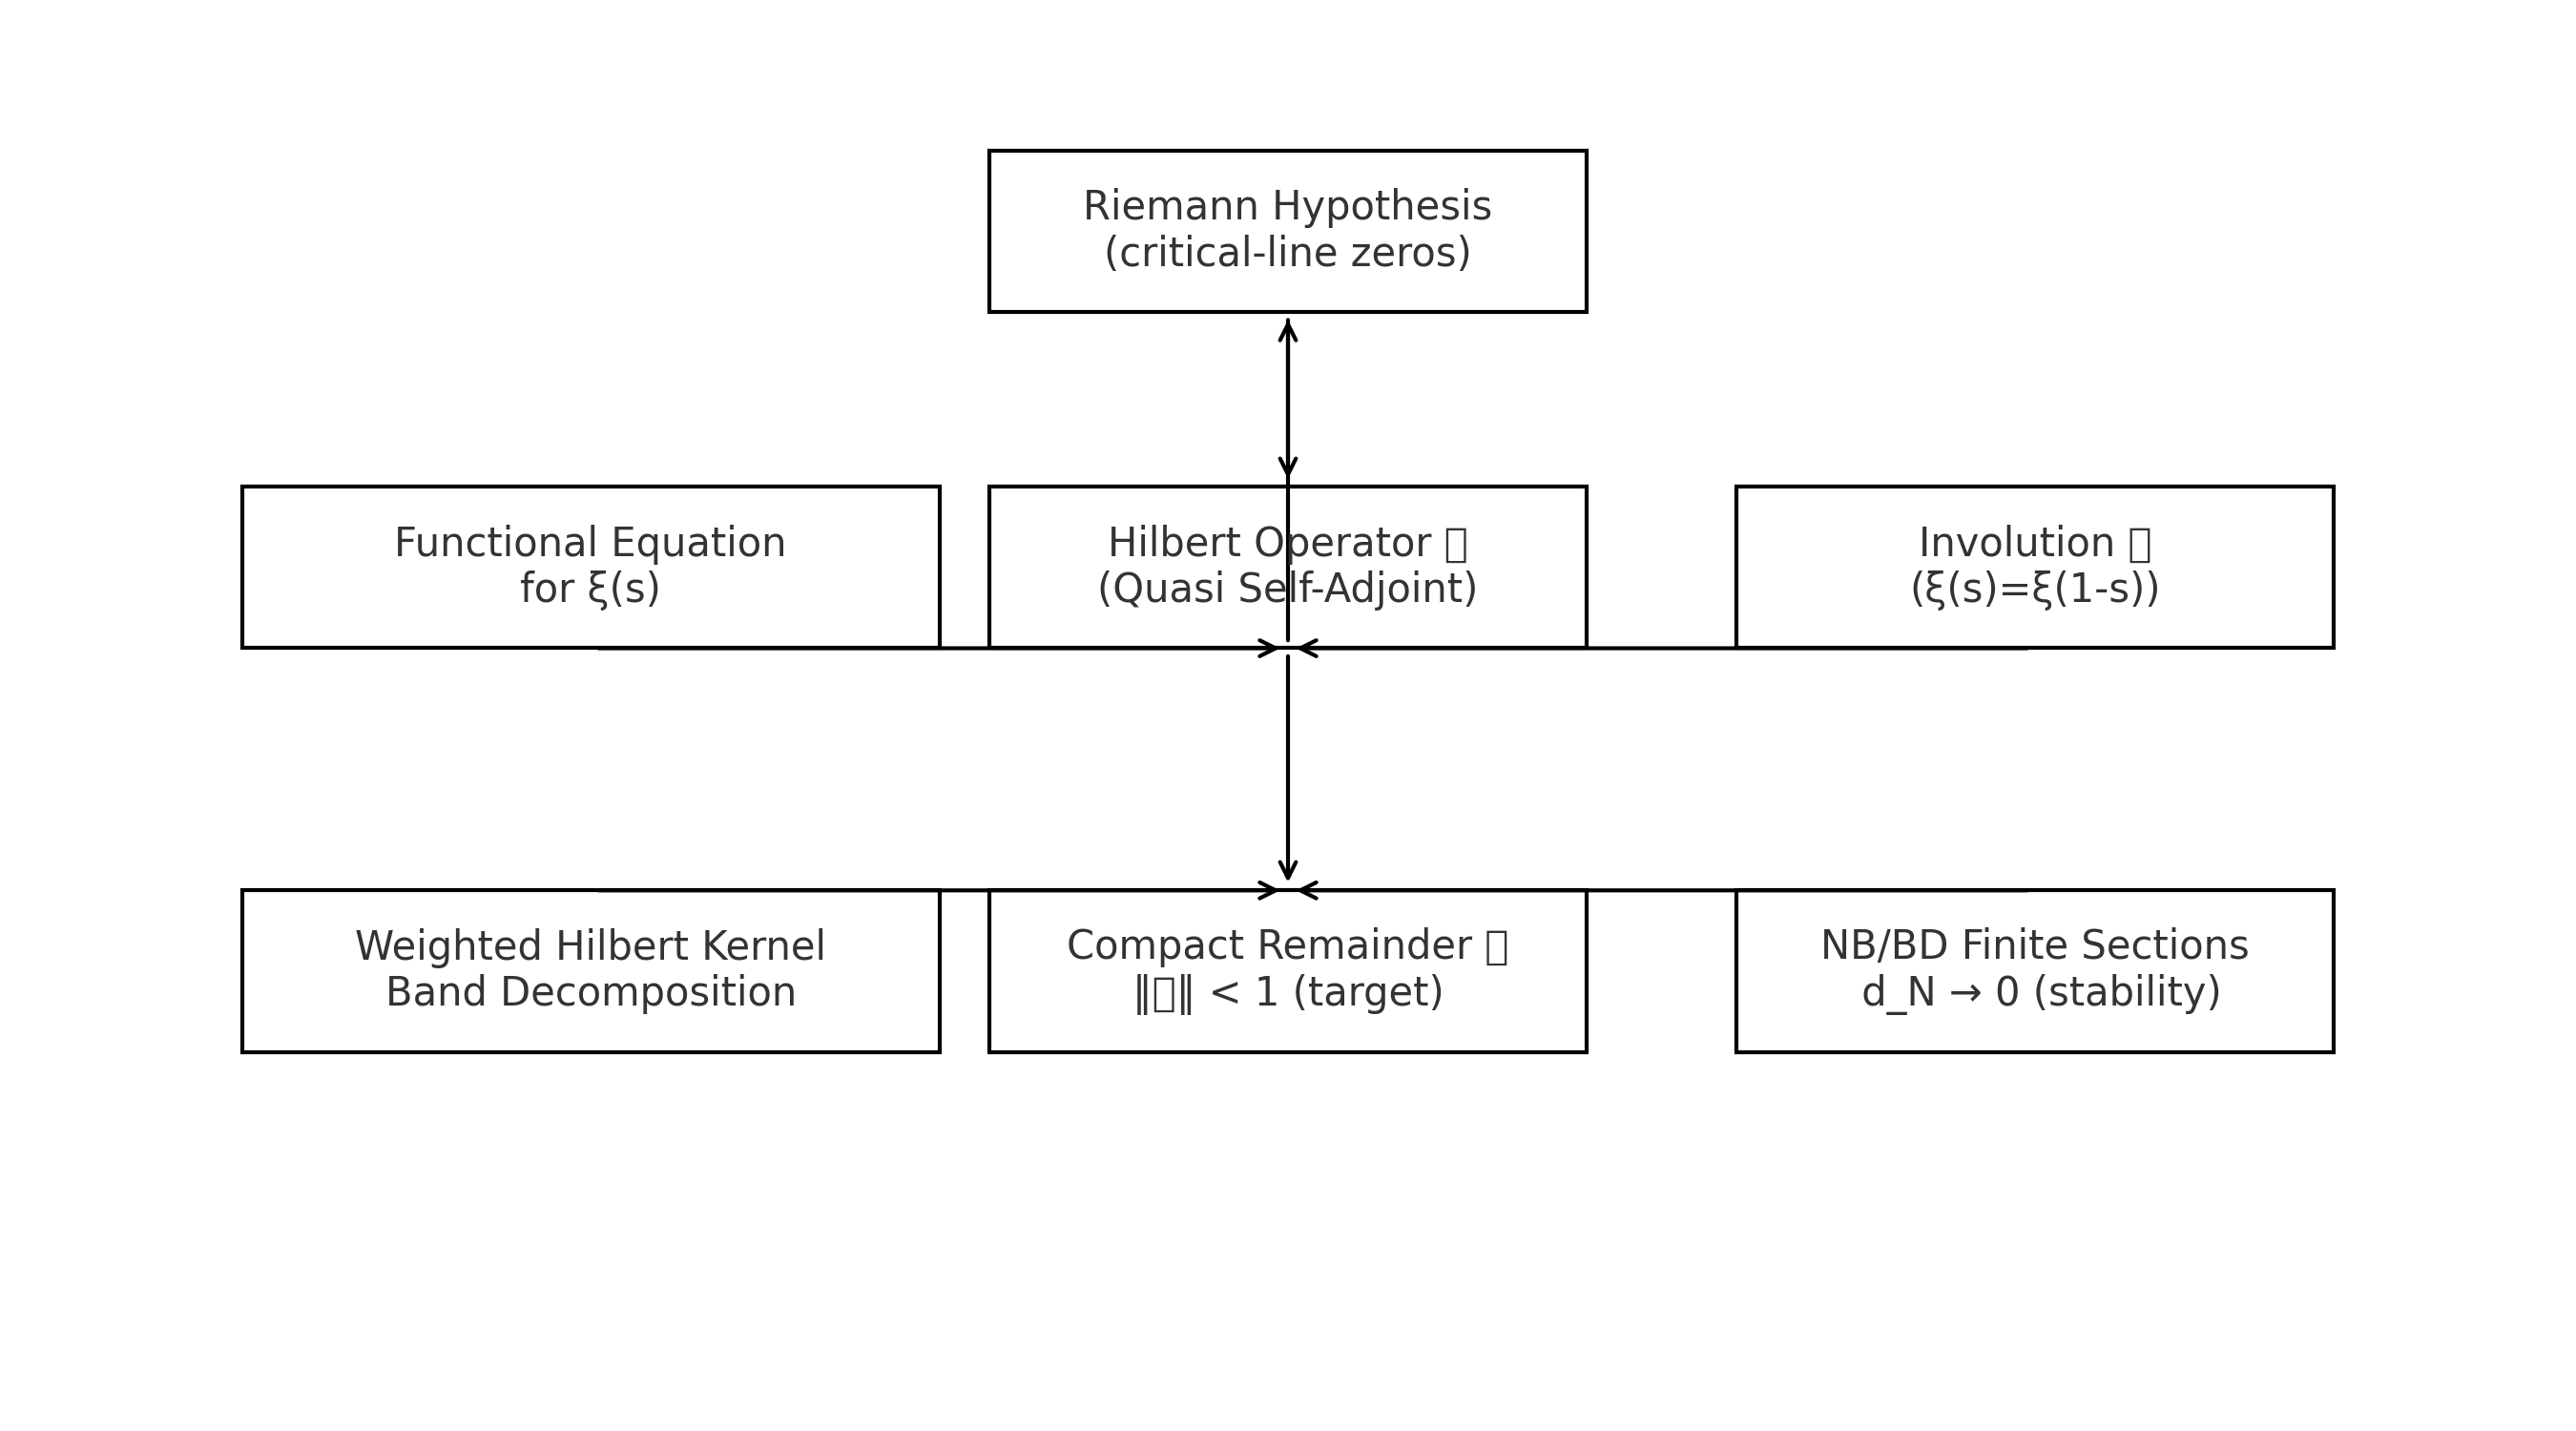
\includegraphics[width=.9\linewidth]{operator_framework_v3_3.png}
\caption{\textbf{Operator roadmap for RH.} Functional symmetry $\Rightarrow$ quasi self-adjoint operator $\mathcal{T}$; weighted Hilbert kernel controls off-diagonal mass; NB/BD sits as a finite-rank surrogate.}
\end{figure}

\paragraph{Disclaimer.}
This note outlines an operator-level pathway and consolidates bounds compatible with NB/BD stability. It is not a proof of RH.

\end{document}
